\begin{figure*}[t]
  \centering
  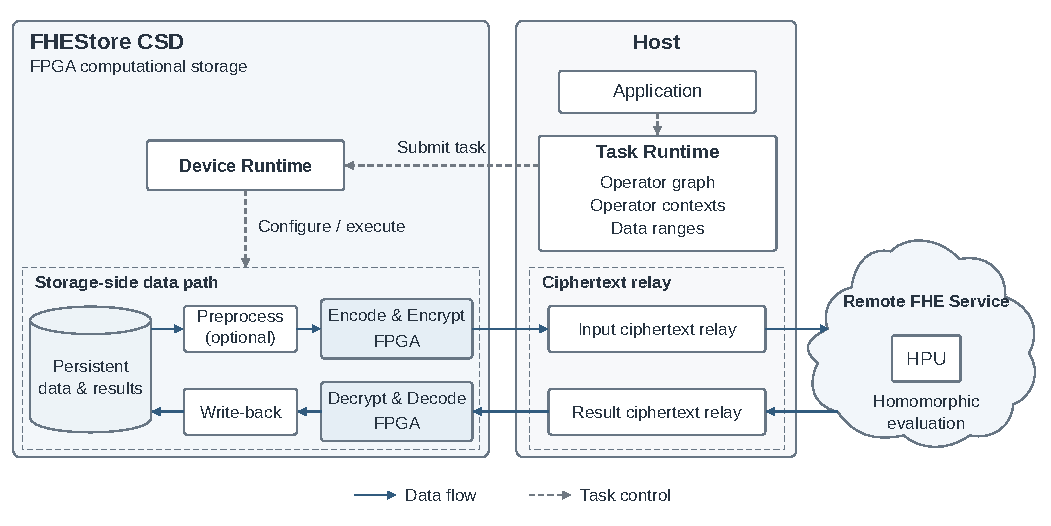
\includegraphics[width=\textwidth]{figures/fhestore-overview-v2/fhestore-overview.pdf}
  \caption{System overview of FHEStore. The host submits an operator graph, per-operator contexts, and data ranges to the device runtime, which configures storage-side execution. Both input ciphertexts and returned result ciphertexts pass through the host relay. Solid arrows denote logical data flow; dashed arrows denote task control. Write-back is a system operation and may include host-assisted read--modify--write.}
  \Description{The diagram has three regions: FHEStore computational storage, the host, and a remote FHE service. The host application passes a task to its runtime, which submits the operator graph, contexts, and data ranges to the device runtime. The device runtime configures storage-side execution. The outbound data path goes from storage through optional preprocessing and FPGA encoding and encryption, then through an input ciphertext relay on the host to the remote HPU service. The return path goes from the service through a result ciphertext relay on the host to FPGA decryption and decoding, write-back, and storage.}
  \label{fig:fhestore-overview}
\end{figure*}
